\documentclass{HW}

\newcommand{\hwtitle}{آزمایش ششم}
\newcommand{\studentname}{رادین شایانفر}
\newcommand{\studentnumber}{9731032}

\usepackage[top=30mm, bottom=30mm, left=25mm, right=25mm]{geometry}
\usepackage{amsthm,amssymb,amsmath,amsfonts}
\usepackage{fancyhdr}
\usepackage{changepage}
\usepackage{enumitem}
\usepackage{listings}
\usepackage[table]{xcolor}
\usepackage{fontspec}

\newfontfamily{\ttconsolas}{Consolas}

\definecolor{codegreen}{rgb}{0,0.6,0}
\definecolor{codegray}{rgb}{0.5,0.5,0.5}
\definecolor{codepurple}{rgb}{0.58,0,0.82}
\definecolor{backcolour}{rgb}{0.95,0.95,0.92}

\lstset{
  backgroundcolor=\color{backcolour},   
  commentstyle=\color{codegreen},
  keywordstyle=\color{magenta},
  numberstyle=\tiny\color{codegray},
  stringstyle=\color{codepurple},
  basicstyle=\ttconsolas\footnotesize,
  breakatwhitespace=false,         
  breaklines=true,                 
  captionpos=b,                    
  keepspaces=true,  
  numbers=left,                    
  numbersep=5pt,                  
  showspaces=false,                
  showstringspaces=false,
  showtabs=false,                  
  tabsize=4
}

\usepackage{array,multirow}

\usepackage{tikz}
\usetikzlibrary{trees}

% بسته‌‌ای برای ظاهر شدن شکل‌ها و تصاویر متن
\usepackage{graphicx}
\usepackage{color}
%بسته‌ای برای تنظیم فاصله عمودی خط‌های متن
\usepackage{setspace}

\usepackage[pagebackref=false,colorlinks,urlcolor=cyan,linkcolor=blue,citecolor=red]{hyperref}

\hypersetup{
    pdftitle={\hwtitle - \studentname - شماره دانشجویی: \studentnumber},
    bookmarks=true,
    pdfauthor={Radin Shayanfar},
}

% بسته‌ لازم برای تنظیم سربرگ‌ها
\usepackage{fancyhdr}

\usepackage{ptext} 
\usepackage{xepersian}

\doublespacing

\SepMark{-}
\settextfont[Scale=1.2]{B Nazanin}
\setlatintextfont{Times New Roman}
\renewcommand{\labelitemi}{$\bullet$}

\newcounter{mynumber}
\setcounter{mynumber}{1}
\newcommand{\mynum}{\arabic{mynumber}\stepcounter{mynumber}}

\newenvironment{question}{%
\medskip%
\par%
\noindent%
\textbf{سوال \mynum- \space}%
\smallskip
%\par\noindent\ignorespaces
\begin{adjustwidth}{7mm}{}
}{%
\end{adjustwidth}
\par\medskip
}

\fancypagestyle{first_page}{
\fancyhf{}
\fancyhead[C]{\raisebox{3ex}{\large \bfseries \hwtitle}}
\fancyhead[LO,LE]{\textbf{\studentname} \\
شماره دانشجویی: \studentnumber
\vspace{0.2mm}}
\fancyfoot[C]{\thepage{}}
\renewcommand{\headrulewidth}{1.2pt}
}

\fancypagestyle{pages}{
\fancyhf{}
\fancyhead[R]{\leftmark}
\fancyfoot[C]{\thepage{}}
\renewcommand{\headrulewidth}{1.2pt}
}

\begin{document}
\pagestyle{pages}
\thispagestyle{first_page}

\section{گام اول}

در این گام، کد ضرب ماتریس‌هایی با حداکثر اندازه ۳۲ در ۳۲ را می‌نویسیم.

در صورتی که در ابتدای برنامه خط

\begin{latin}
%\begin{minipage}{\linewidth}
\begin{lstlisting}[language=C, belowskip=-0.5\baselineskip]
#define DEBUG
\end{lstlisting}
%\end{minipage}
\end{latin}

قرار گیرد، نتایج محاسبات پس از اجرای کرنل و پیش از آزادسازی حافظه‌ها بر روی میزبان (\lr{CPU}) به شکل تک‌نخی بررسی می‌شود. اگر ضرب ماتریس‌ها نادرست انجام شده باشد، در این قسمت پیغام \lr{wrong answer} چاپ می‌شود.


\section{گام دوم}

در این گام سه راه‌حل مختلف برای ضرب ماتریس‌ها پیاده‌سازی شده است. در روش اول تنها ۱۰۲۴ نخ در یک بلوک تمام محاسبات را انجام می‌دهند. این روش در کرنل \lr{matMulA1Kernel} پیاده‌سازی شده است. روش دوم که در کرنل \lr{matMulA2Kernel} پیاده شده است، به تعداد درایه‌های ماتریس‌ها نخ در بلوک‌های مختلف اختصاص می‌دهد. در روش سوم و آخر از تکنیک \lr{tiling} با اندازه بلوک و کاشی‌های ۳۲ در ۳۲ استفاده شده است. روش سوم نیز در کرنل \lr{matMulA3Kernel} آمده است.

در ابتدای برنامه با تغییر خط
\begin{latin}
%\begin{minipage}{\linewidth}
\begin{lstlisting}[language=C, belowskip=-0.5\baselineskip]
#define APPROACH x
\end{lstlisting}
%\end{minipage}
\end{latin}
می‌توان برنامه را با راه‌حل شماره \lr{x} اجرا کرد.


\begin{table}[ht]
\caption{زمان‌های اجرا (میلی ثانیه) به ازای اندازه ورودی‌های مختلف}
\begin{center}
\begin{tabular}{|c|c|c|c|c|}
    \hline
    \multirow{2}{*}{موازی‌سازی} & \multicolumn{3}{|c|}{اندازه ورودی}& \multirow{2}{*}{تسریع} \\
    \cline{2-4}
& $2^{10}$ & $2^{11}$ & $2^{12}$ & \\
    \hline
  سریال & 
  1753/2 & 56280/0 & 538651/5 & - \\ \hline
  
راه‌حل اول &
  687/8 & 6011/7 & 53455/7 &  \\ \hline
  
راه‌حل دوم & 
  8/5 & 68/7 & 622/0 &  \\ \hline
 
 راه‌حل سوم (کاشی‌کاری) & 
  8.8 & 69.9 & 592/8 &  \\ \hline
\end{tabular}
\end{center}
\label{tab:section2-results}
\end{table}

\begin{table}[ht]
\caption{زمان‌های اجرا (میلی ثانیه) به ازای اندازه ورودی‌های مختلف}
\begin{center}
\begin{tabular}{|c|c|c|c|c|}
    \hline
    \multirow{2}{*}{موازی‌سازی} & \multicolumn{3}{|c|}{اندازه ورودی}& \multirow{2}{*}{تسریع} \\
    \cline{2-4}
& $2^{10}$ & $2^{11}$ & $2^{12}$ & \\
    \hline
  کاشی‌کاری با حافظه مشترک & 
  8/2 & 61/5 & 515/3 &  \\ \hline

\end{tabular}
\end{center}
\label{tab:section3-results}
\end{table}



%\begin{figure}[ht!]
%\begin{center}
%	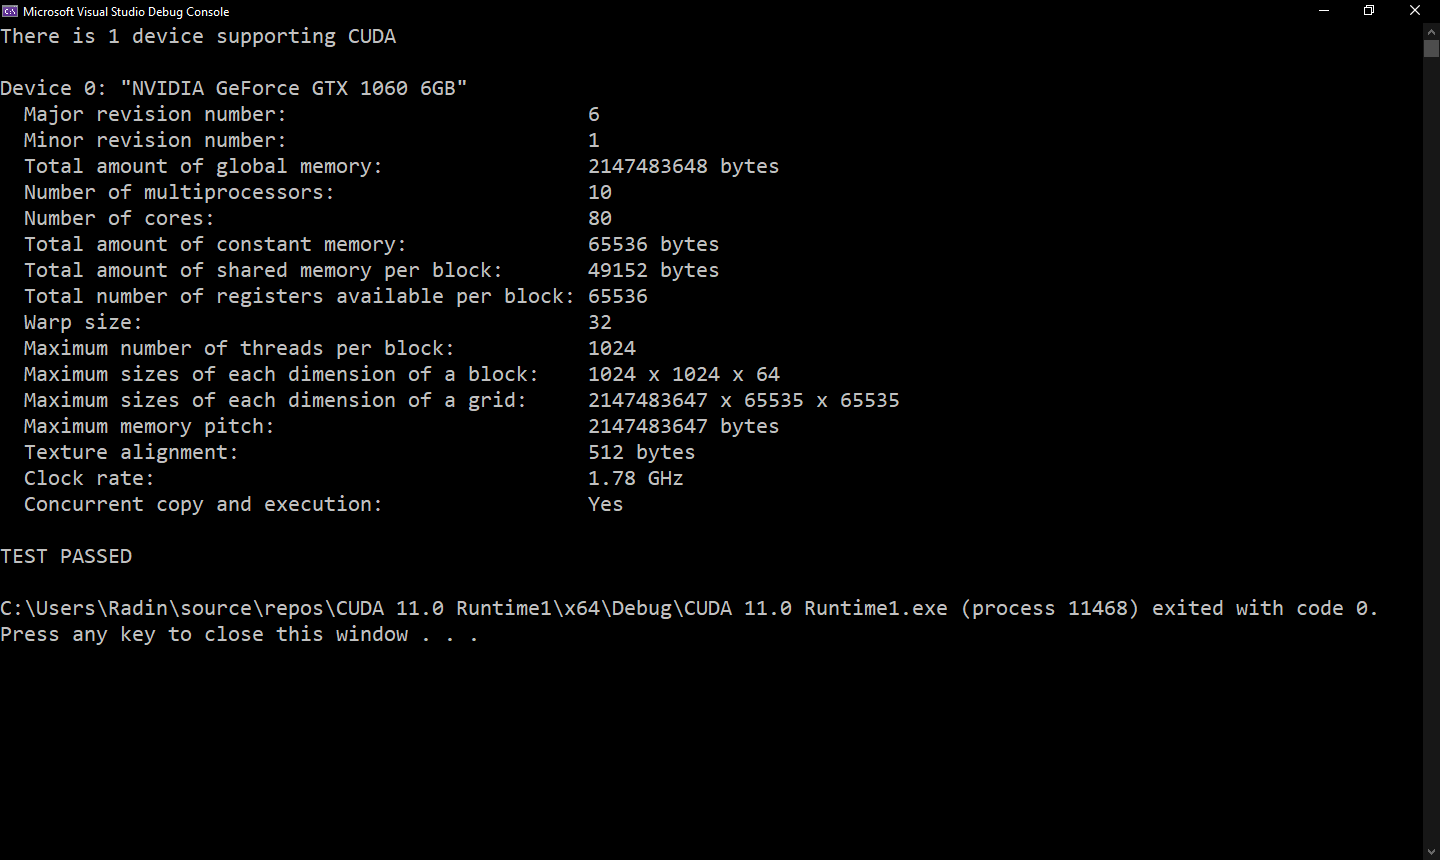
\includegraphics[width=15cm]{images/query}
%\end{center}
%\caption{مشخصات دستگاه با استفاده از کد \lr{deviceQuery}}
%\label{fig:query}
%\end{figure}


\end{document}
